\documentclass[11pt,a4paper]{article}
\usepackage[utf8]{inputenc}
\usepackage[hmargin=2.0cm,vmargin=2.5cm,bindingoffset=0.5cm]{geometry}
\usepackage{amsfonts}
\usepackage{amsmath,amsthm,amssymb}
\allowdisplaybreaks
\usepackage{hyperref}
\usepackage{graphicx}
\usepackage{tikz}
\usepackage{mathtools}
\DeclarePairedDelimiter\ceil{\lceil}{\rceil}
\DeclarePairedDelimiter\floor{\lfloor}{\rfloor}
%\usepackage{float}
\usepackage{placeins}
\usepackage{diagbox}
\DeclareMathOperator{\Tr}{Tr}
\newtheorem{thm}{Theorem}
\usepackage{subcaption}
%\usepackage{subfigure}
\usepackage[english]{babel}
\author{Mohit}
\title{Quantum control of NV center using counter-diabatic driving  }
\begin{document}
\maketitle
%\tableofcontents

\section{Introduction}
The ground state of the NV center is a spin triplet with $| 0 \rangle, | -1 \rangle, | 1 \rangle$ spin sub-levels. They are defined in $S_z$ basis , where $\hat{z}$ direction is along the NV center axis. The Hamiltonian for the ground state of the NV center can be written as \cite{dhingra2017nitrogen}:
\begin{equation}
H_{NV}= \hbar \Delta S_z^2 + g \mu_B \vec{S}. \vec{B}_{ext} 
\end{equation}
where $\Delta= 2 \pi \times 2.87 $ GHz is zero-field splitting, $g \approx 2$ is the g-factor of electron in the NV center and $\mu_B$ is Bohr magneton. If there is no external magnetic field, then $| -1 \rangle$ and $| 1 \rangle$ levels are degenerate, and  $ \hbar^3 \Delta$ is the energy difference between $| 0 \rangle$ and $| \pm 1 \rangle$ energy levels.


Let's choose magnetic field to be in x-direction. Then we have:
\begin{align*}
H_{NV} &= \hbar \Delta S_z^2 + g \mu_B   S_x  B \\
 &= \Lambda S_z^2 + \lambda   S_x  
\end{align*}
where $\Lambda= \hbar \Delta $ and $\lambda=g \mu_B    B $. Magnetic field is going to be our control parameter in this problem. Using spin algebra, we obtain Hamiltonian in the basis ($|- 1\rangle$, $| 0 \rangle$ , $| 1 \rangle$):

\begin{equation}
H= \begin{bmatrix}
    \beta       & \alpha  & 0  \\
    \alpha       & 0 &\alpha  \\
     0       & \alpha & \beta
\end{bmatrix}
\end{equation}
where $\alpha= \hbar \lambda/ \sqrt{2} $ and $\beta= \hbar^2 \Lambda$.


\begin{figure}[!ht]
\begin{center}
\includegraphics[scale=0.5]{pics/energy_level_beta1.eps} 
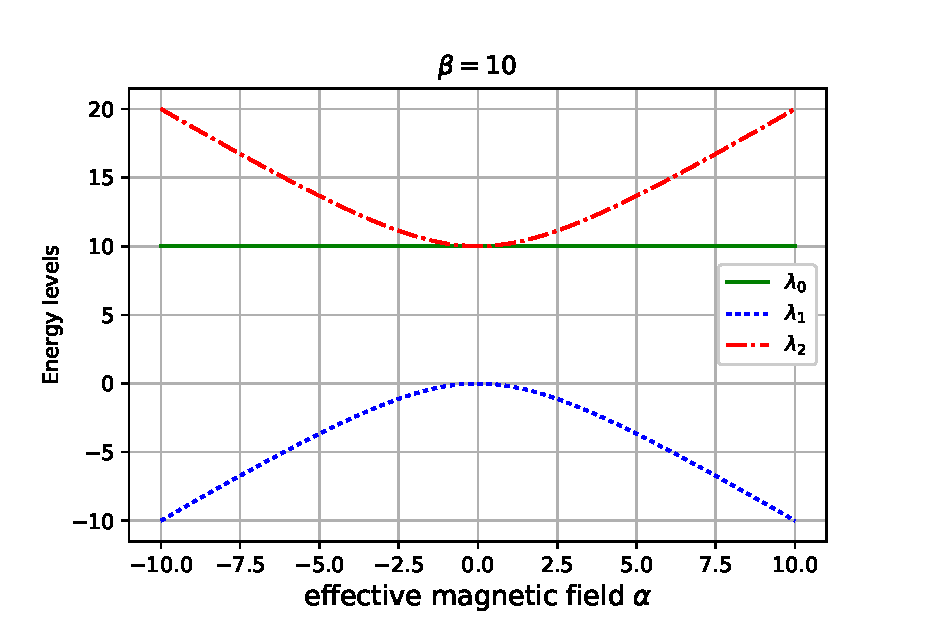
\includegraphics[scale=0.5]{pics/energy_level_beta10.eps} 
\caption{Avoided level crossing as a function of effective magnetic field }
\label{ev}
\end{center}
\end{figure}

 Energy eigenvalues are given by:
\begin{align*}
\lambda_0 &= \beta, \quad \lambda_1 = (\beta - \sqrt{\beta^2 + 8 \alpha^2})/2 , \quad  \lambda_2 = (\beta + \sqrt{\beta^2 + 8 \alpha^2})/2
\end{align*}
We should remember that $\alpha \propto B$. Hence, it makes sense that when $\alpha=0$,  there is a two -fold degeneracy and zero field energy gap is given by $\beta=\hbar^3 \Delta$. Now let's have a look at eigenvectors:
\begin{align*}
\nu_0 = (-1,0,1), \quad \nu_1 = (1, -(\beta + \sqrt{\beta^2 + 8 \alpha^2})/2 \alpha, 1) , \quad \nu_2 = (1, -(\beta - \sqrt{\beta^2 + 8 \alpha^2})/2 \alpha, 1)
\end{align*}



Now let's compute gauge potential:

Let's find out $A_{\lambda}$ for this Hamiltonian for which we need to compute different odd-powered commutator $[H, \partial_{\lambda} H]$, where $\partial_{\lambda} H=S_x$. Here we begin:
\begin{align*}
C^{(1)}=[H,S_x] &= \Lambda  [S_z^2, S_x] \\
&= S_z[S_z, S_x] + [S_z, S_x] S_z \\
&= 2i \hbar (S_z S_y + S_y S_z) \\
&=2i \hbar ([S_z, S_y] +  2 S_y S_z)\\
&=2i \hbar (- i \hbar S_x +  2 S_y S_z)
\end{align*}

\begin{align*}
C^{(2)}=[H,C^{(1)}] &=    -2 \hbar^2 [H,  S_x]  + 2[ H,   S_y S_z] \\
&= -2 \hbar^2 C^{(1)}  + 2 S_y[ H,    S_z] + 2[ H,   S_y ]S_z\\
&= -2 \hbar^2 C^{(1)}  + 2 \lambda S_y [ S_x,    S_z] + T\\
&= -2 \hbar^2 C^{(1)}  - 2i \hbar \lambda S_y^2  + T
\end{align*}

\begin{align*}
T=2[ H,   S_y ]S_z &= \Lambda [S_z^2, S_y]S_z + \lambda   [S_x, S_y]S_z   \\
 &=   \Lambda S_z[S_z, S_y]S_z+\Lambda [S_z, S_y]S_z^2 + 2 i \hbar \lambda   S_z^2   \\
  &=  -2i \Lambda  ( S_z S_x S_z+ S_x S_z^2) + 2 i \hbar \lambda   S_z^2   \\
    &=  -2i \Lambda  ( [S_z, S_x] S_z+ 2 S_x S_z^2) + 2 i \hbar \lambda   S_z^2   \\
        &=  -4i \Lambda  ( i S_y S_z+  S_x S_z^2) + 2 i \hbar \lambda   S_z^2   
\end{align*}
Hence, we get:
\begin{align*}
C^{(2)}=[H,C^{(1)}]  &= -2 \hbar^2 C^{(1)}  - 2i \hbar \lambda (S_y^2 -S_z^2)  -4i \Lambda  ( i S_y S_z+  S_x S_z^2) 
\end{align*}
Further, 
\begin{align*}
C^{(3)}=[H,C^{(2)}] &= [H,-2 \hbar^2 C^{(1)}  - 2i \hbar \lambda (S_y^2 -S_z^2)  -4i \Lambda  ( i S_y S_z+  S_x S_z^2)] \\
&= -2 \hbar^2  C^{(2)} - 2i \hbar \lambda [H,(S_y^2 -S_z^2)]  -4i \Lambda  [H,( i S_y S_z+  S_x S_z^2)] 
\end{align*}

\appendix
\section{Spin Algebra}\label{sec.spin_alegbra}
\begin{equation}
S^2|s ,m \rangle = \hbar^2 s(s+1)|s ,m\pm 1\rangle  \quad S_z|s ,m \rangle = \hbar m |s ,m \rangle
\end{equation}
\begin{align*}
S_{\pm}|s, m\rangle = \hbar\sqrt{s(s+1)-m(m \pm 1)}|s,m \pm 1\rangle
\end{align*}
where $S_+ = S_x + iS_y$ and $S_- = S_x - iS_y $. Hence, we get $S_x = (S_+ + S_-)/2$ and $S_y = (S_+ - S_-)/2i $
\bibliography{ref} 

\bibliographystyle{unsrt}
%\bibliographystyle{plain}

\end{document}
